\section{Testvorbereitung}
Wir w�hlen die InnoDB als Speichermaschine aus, da sie die Transaktionssicherheit gew�hrleistet und sich dadurch f�r das Betreiben eines Webshops am besten eignet. 
Jede Versuchsreihe entspricht einer bestimmten Konfiguration und besteht aus vier Testl�ufen zu je einem Use Case. Am Anfang  werden Testdaten mit einer  bestimmten Anzahl von Kunden, einer konstanten Anzahl von Produkten (1000), einer konstanten Anzahl von Warenk�rben pro Kunde(5) und genauso einer konstanten Anzahl von Produkten pro Warenkorb(5) generiert. Die Anzahl der Kunden erh�ht sich mit jedem Testlauf. In jeder Versuchsreihe werden die vier verschiedenen Use Cases betrachtet, die durch eine unterschiedliche SELECT-Anweisung an die MySQL-Datenbank realisiert werden:
\subsection{SELECT-Anweisungen}
\begin{enumerate}
\item \textbf{Use Case 1: Welches Produkt wurde wie oft gekauft?}
\lstset{language=Java,caption={UseCase1},label=Use Case 1}
\lstinputlisting[language=Java]{Christof/Listings/UseCase1.java}
\item \textbf{Wieviel Umsatz wurde von wem in bestimmtem Zeitraum generiert?}
\lstset{language=Java,caption={UseCase2},label=Use Case 2}
\lstinputlisting[language=Java]{Christof/Listings/UseCase2.java}
\item \textbf{Wie viele Kunden haben in bestimmten Zeitraum bestellt?}
\lstset{language=Java,caption={UseCase3},label=Use Case 3}
\lstinputlisting[language=Java]{Christof/Listings/UseCase2.java}
\item \textbf{Wie viel Umsatz wurde an den ersten drei Tagen der ersten drei Monate generiert?}
\lstset{language=Java,caption={UseCase4},label=Use Case 4}
\lstinputlisting[language=Java]{Christof/Listings/UseCase2.java}
\end{enumerate}

\subsection{Konfigurationen der MySQL-Datenbank und der Tabellen}
Jede Versuchsreihe testet die SELECT-Anweisungen mit einer bestimmten Konfiguration der MySQL-Datenbank und der Tabellen. Vor jedem Testlauf werden die entsprechenden Konfigurationseintellungen mit SQL-Anweisungen durchgef�hrt.
\begin{enumerate}
\item \textbf{K1} : Kaltstart ohne Index
\item \textbf{K2} : Warmstart ohne Index
\item \textbf{K3} : Hash-Indizes auf Primary Keys und Foreign Keys / ohne Partitioning
\item \textbf{K4} : B-Tree-Indizes auf Primary Keys und Foreign Keys / ohne Partitioning
\item \textbf{K5} : Hash-Indizes auf Primary Keys und Foreign Keys sowie B-Tree-Index auf Datum / ohne Partitioning
\item \textbf{K6} : Hash-Indizes auf Primary Keys und Foreign Keys sowie B-Tree-Index auf Datum / mit List-Partitioning auf MONTH(Datum) f�r jedes Quartal
\item \textbf{K7} : Hash-Indizes auf Primary Keys und Foreign Keys sowie B-Tree-Index auf Datum / mit Hash-Partitioning auf MONTH(Datum) f�r jeden Monat
\item \textbf{K8} : Hash-Indizes auf Primary Keys und Foreign Keys sowie B-Tree Index auf Datum / mit Range-Partitioning auf COLUMNS(Datum) f�r jedes Quartal
\item \textbf{K9} : Hash Indizes auf Primary Keys und Foreign Keys sowie B-Tree-Index auf Datum / mit Sub-Partitioning (Range-Partitioning quartalsweise auf Datum und f�r jedes Quartal jeweils vier Hash-Partitions auf TO\_DAYS(Datum))
\item \textbf{K10}: Hash-Indizes auf Primary Keys und Foreign Keys / mit Sub-Partitioning (Range-Partitioning quartalsweise auf Datum und f�r jedes Quartal jeweils vier Hash-Partitions auf TO\_DAYS(Datum)
\end{enumerate}

\subsection{EXPLAIN-Anweisung}
Bei den SQL-Abfragen stellten wir bei jeder SELECT-Anweisung ein EXPLAIN davor, um n�tzliche Informationen zum Ausf�hrungsplan des Optimierers zu erhalten. Die EXPLAIN-Anweisung liefert u.a. Daten dar�ber, ob die Indizes auch wirklich benutzt wurden, in welcher Reihenfolge die Tabellen verkn�pft werden sowie weitere Informationen, die helfen sollen die SELECT-Anweisungen zu beschleunigen.  
\subsection{EXPLAIN PARTITIONS-Anweisung}
Diese Anweisung liefert zus�tzlich Informationen �ber die verwendeten Partitionen. Man kann sie jedoch nur auf RANGE- oder LIST-partitionierte Tabellen verwenden. Bei KEY- oder HASH-Partitionen ist sie unbrauchbar, da automatisch alle Partitionen ausgegeben werden. 

\section{Testdurchf�hrung}

\subsection{Behauptung}

\subsection{Testergebnisse bei 1 Mio. Kunden}
\begin{figure}[htp]
\centering
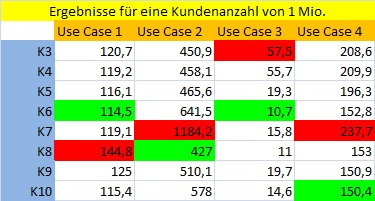
\includegraphics[width=0.75\textwidth]{Christof/Bilder/auswert1.jpg}
\caption{Testergebnisse}
\label{fig:auswert1}
\end{figure}

\subsection{Testauswertung}





